\section{Repetições}
\index{Música!Repetições}
\label{sec:repetitions}

\subsection{Repetições de compassos}
\index{Música!Repetições de compassos}
\label{sec:repetitions:compass}

É possivel expressar a repetição de um o mais compassos usando o simbolo $\%$ 
\cite[pp. 249]{medteoria} \cite[pp. 111]{mascarenhascurso}.
A Figura \ref{fig:repeat-bar1-1} mostra o uso de repetições para escrever de forma compacta uma melodia.
A Figura \ref{fig:repeat-bar2-1} mostra a forma expandida da melodia expressada na Figura \ref{fig:repeat-bar1-1}.
\begin{figure}[!h]
\centering
    \begin{subfigure}[b]{0.6\textwidth}
        \includegraphics[width=0.9\textwidth]{chapters/cap-musica-basica/repeat-bar1-1.eps}
        \caption{Forma compacta.}
        \label{fig:repeat-bar1-1}
    \end{subfigure}
    \begin{subfigure}[b]{0.6\textwidth}
        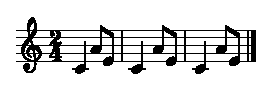
\includegraphics[width=0.9\textwidth]{chapters/cap-musica-basica/repeat-bar2-1.eps}
        \caption{Forma expandida.}
        \label{fig:repeat-bar2-1}
    \end{subfigure}
\caption{Uso de repetições de compassos.}
\label{fig:repeat-bar1}
\end{figure}


\subsection{Repetições de trechos musicais}
\index{Música!Repetições de trechos}
\label{sec:repetitions:manycompass}

\subsubsection{Ritonelo}
\index{Música!Ritonelo}
É possivel expressar a repetição de um trecho de música usando o ``ritnonelo'' 
que tem um simbolo ``$:|$'' \cite[pp. 237]{medteoria} \cite[pp. 168]{cardoso1973curso}.

\begin{example}[Uso de ritnonelo final:]Se temos uma melodia com compasses $A$, $B$ e $C$,
então estas duas formas são equivalentes:
\begin{itemize}
\item $A~B~C~:|$
\item $A~B~C~A~B~C$
\end{itemize}
\end{example}


\begin{example}[Uso de ritnonelo inicial final:]Se temos uma melodia com compasses $A$, $B$ e $C$,
então estas duas formas são equivalentes:
\begin{itemize}
\item $ A|:B~C:|$
\item $A~B~C~B~C$
\end{itemize}
\end{example}

A Figura \ref{fig:ritonelo1-1} mostra o uso de repetições para escrever de forma compacta uma melodia.
A Figura \ref{fig:ritonelo2-1} mostra a forma expandida da melodia expressada na Figura \ref{fig:ritonelo1-1}.
\begin{figure}[!h]
\centering
    \begin{subfigure}[b]{0.75\textwidth}
        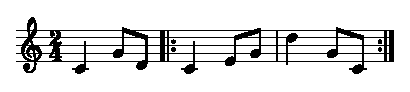
\includegraphics[width=0.9\textwidth]{chapters/cap-musica-basica/ritonelo1-1.eps}
        \caption{Forma compacta.}
        \label{fig:ritonelo1-1}
    \end{subfigure}
    \begin{subfigure}[b]{0.75\textwidth}
        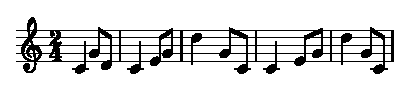
\includegraphics[width=0.9\textwidth]{chapters/cap-musica-basica/ritonelo2-1.eps}
        \caption{Forma expandida.}
        \label{fig:ritonelo2-1}
    \end{subfigure}
\caption{Uso de repetições de trechos de música.}
\label{fig:ritonelo1}
\end{figure}

\subsubsection{Ritonelo com expressoes de 1ra e 2da vez}
Se um trecho de musica deve ser repetido mas com um diferente final cada vez,
então deve ser usado a expressão ``1ra vez'' e ``2da vez''
\cite[pp. 239]{medteoria} \cite[pp. 169]{cardoso1973curso}.

A Figura \ref{fig:ritonelo-times1-1} mostra o uso de repetições para escrever de forma compacta uma melodia.
A Figura \ref{fig:ritonelo-times2-1} mostra a forma expandida da melodia expressada na Figura \ref{fig:ritonelo-times1-1}.
\begin{figure}[!h]
\centering
    \begin{subfigure}[b]{0.75\textwidth}
        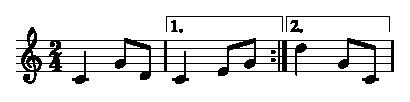
\includegraphics[width=0.9\textwidth]{chapters/cap-musica-basica/ritonelo-times1-1.eps}
        \caption{Forma compacta.}
        \label{fig:ritonelo-times1-1}
    \end{subfigure}
    \begin{subfigure}[b]{0.75\textwidth}
        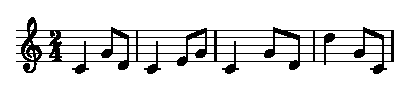
\includegraphics[width=0.9\textwidth]{chapters/cap-musica-basica/ritonelo-times2-1.eps}
        \caption{Forma expandida.}
        \label{fig:ritonelo-times2-1}
    \end{subfigure}
\caption{Uso de repetições de trechos de música com expressoes de vez.}
\label{fig:ritonelo-times1}
\end{figure}

